\documentclass[11pt]{article}
\usepackage[margin=1in]{geometry}
\usepackage{booktabs}
\usepackage{amsmath}
\usepackage{enumitem}
\usepackage[hidelinks]{hyperref}
\usepackage{parskip}
\usepackage{graphicx}

\title{AI-Powered Marketing Budget Allocation Agent\\
\large Final Project Report --- MGMT 590-037 $\cdot$ AI-Enhanced Optimization\\
Daniels School of Business, Purdue University $\cdot$ Summer 2026}
\author{Ana Valderrama $\cdot$ Gregory Sapp $\cdot$ Meghna Advani $\cdot$ Piyush Sandhikar $\cdot$ Vikhyat Koppal}
\date{June 2026}

\begin{document}
\maketitle

\section*{Executive Summary}

We built an AI agent that converts five years of real eCommerce marketing data into a weekly, dollar-level budget recommendation across five paid advertising channels --- and explains, defends, and stress-tests that recommendation in plain language. The agent follows the course's \textbf{Data $\rightarrow$ Prediction $\rightarrow$ Optimization $\rightarrow$ Decision} pipeline end-to-end: it cleans and validates 132{,}759 rows of daily channel data, fits saturating response curves per channel, tunes the model's hyperparameters with Bayesian Optimization, and solves a constrained nonlinear allocation problem with verified optimality conditions.

The headline result: at a demonstration budget of \$50{,}000 per week, the optimized allocation predicts \textbf{15{,}640.8 conversions versus 5{,}957.1} for the proportional-to-history status quo --- a \textbf{+162.6\% lift from reallocation alone}, with no additional spend. The agent also reports the budget's shadow price (0.30 conversions per marginal dollar), a budget-sensitivity grid showing diminishing returns, and honest diagnostics about which channel estimates are well-identified and which are not. Under the instructor's stakeholder modification --- minimum activation thresholds and advertising carryover --- the problem becomes non-convex; the agent restores a provably global optimum by enumerating all 32 channel ON/OFF patterns and solving a convex subproblem within each.

Our recommendation to a marketing executive is direct: \emph{reallocate before you spend more}. The marginal dollar belongs to the channel with the highest marginal response until marginal returns equalize --- and the agent computes exactly where that point is, every week, in milliseconds.

\section{Problem Description and Motivation}

\subsection{The decision problem}

A mid-market direct-to-consumer (DTC) eCommerce brand spends roughly \$831{,}000 per week on paid media across five channels: Google Paid Search, Google Shopping, Google Performance Max (PMax), Meta Facebook, and Meta Instagram. Every week, someone must decide how to split that budget. The decision recurs 52 times a year and individual channels consume tens of thousands of dollars weekly, yet in most organizations it is made by proportional rollover of last quarter's ROAS, platform-reported attribution, or managerial intuition.

\subsection{Why current practice fails}

Three structural features of paid digital advertising defeat these heuristics:

\begin{enumerate}[nosep]
  \item \textbf{Saturating response.} Channel response is concave: the first dollar buys far more conversions than the millionth. ROAS-ranked allocation funds ``winning'' channels straight into their saturation zone while starving channels with high marginal returns.
  \item \textbf{Carryover (adstock).} Impressions served this week continue converting in later weeks. Single-period attribution under-credits channels with long decay.
  \item \textbf{Activation thresholds.} Platforms have minimum effective spends $\kappa_c$ below which campaigns never reach audience frequency. The real decision is not only \emph{how much} per channel but \emph{whether to run a channel at all} --- a disjunctive, non-convex structure no spreadsheet heuristic handles.
\end{enumerate}

\subsection{From prediction to prescription}

A standard analytics pipeline would stop at prediction: ``Google Shopping converts well.'' That is a forecast, not a decision. The gap between the two is exactly what this project closes. Prediction gives us each channel's \emph{response curve} --- conversions as a function of spend. Prescription requires embedding those curves in an optimization model with a budget, bounds, and activation logic, then solving for the spend vector that maximizes total predicted conversions. The agent automates the full chain and returns dollar amounts, not sentiments.

\section{Problem Formulation}

Following the backward-thinking discipline used throughout the course, we state the decision problem formally before touching any data.

\subsection{Decision variables}

\[
s = (s_1, \dots, s_5), \qquad s_c \ge 0 \;\; \text{(weekly USD spend on channel } c\text{)}
\]

one variable per modeled channel: Google Paid Search, Google Shopping, Google PMax, Meta Facebook, Meta Instagram. The decision cadence is weekly.

\subsection{Objective function}

Maximize total predicted weekly conversions, where each channel contributes through a concave saturation curve:

\[
\max_{s} \;\; Z(s) = \sum_{c=1}^{5} a_c\left(1 - e^{-b_c s_c}\right)
\]

$a_c$ is the channel's conversion ceiling and $b_c$ its saturation rate. The functional form encodes three business facts: zero spend yields zero incremental conversions, the marginal return $a_c b_c e^{-b_c s_c}$ is highest at low spend, and returns approach a finite ceiling. Both parameters are \emph{uncertain} and must be estimated from data --- this is the prediction task.

\subsection{Constraints}

\begin{center}
\begin{tabular}{lll}
\toprule
\textbf{Constraint} & \textbf{Form} & \textbf{Business meaning} \\
\midrule
Budget & $\sum_c s_c \le B$ & Total weekly spend cannot exceed the budget \\
Ceilings & $s_c \le u_c$ & No channel exceeds $1.5\times$ its historical weekly max \\
Non-negativity & $s_c \ge 0$ & Spend cannot be negative \\
Activation (Models B, C) & $s_c \in \{0\} \cup [\kappa_c, u_c]$ & Run a channel at minimum effective scale, or not at all \\
\bottomrule
\end{tabular}
\end{center}

The activation constraint is the instructor's stakeholder modification. It makes the feasible set a disjoint union --- the problem is non-convex and cannot be handled by a single local solve (Section 6).

\subsection{Backward mapping: Decision $\rightarrow$ Parameters $\rightarrow$ Data $\rightarrow$ Prediction $\rightarrow$ Optimization}

\begin{center}
\begin{tabular}{ll}
\toprule
\textbf{Layer} & \textbf{Content} \\
\midrule
Decision & Allocate budget $B$ across five channels, weekly, in dollars \\
Parameters needed & $(a_c, b_c)$ response curves; adstock decays $\lambda_c$; thresholds $\kappa_c$; ceilings $u_c$; budget $B$ \\
Data to estimate them & Five years of daily per-channel spend, impressions, clicks, and purchases \\
Prediction layer & Weekly Marketing Mix Model (MMM) on adstocked spend, hyperparameters tuned by BO \\
Optimization layer & Constrained nonlinear maximization; activation-pattern enumeration when non-convex \\
\bottomrule
\end{tabular}
\end{center}

Each layer exists \emph{because} the layer above it demands something: the decision demands curve parameters, the parameters demand historical spend--response data, the data demands a principled estimator, and the estimates demand an optimizer that respects the constraints a marketer actually faces.

\section{Data Sources and Preparation}

\subsection{Dataset and structure}

We use the \textbf{Multi-Region Marketing Mix Modeling Dataset} published by Conjura (figshare ID 25314841) --- real, public, and fully disclosed, per the course's no-synthetic-data requirement. Coverage: \textbf{132{,}759 daily rows $\times$ 50 columns}, 93 anonymized eCommerce brands across 15 verticals and 14 currencies, spanning 21 July 2019 to 2 June 2024.

The 50 columns fall into four groups:

\begin{itemize}[nosep]
  \item \textbf{Identifiers:} anonymized company, country, vertical, and date --- each (company, country) pair is one daily timeseries.
  \item \textbf{Channel activity:} spend, impressions, and clicks per channel for Google (Paid Search, Shopping, PMax, Display, Video), Meta (Facebook, Instagram, Other), and TikTok.
  \item \textbf{Outcomes:} transactions and revenue --- total and new-customer --- from which we build the conversion target $y$.
  \item \textbf{Commercial context:} currency, average order values, and related descriptors used for normalization and audit.
\end{itemize}

\subsection{Channel selection: which channels we kept, and why}

Modeling a channel requires enough non-null spend history to fit a response curve. An explicit null-rate audit drove the keep/drop decision, and the agent surfaces this reasoning to the user in its live data-quality stage rather than burying it in preprocessing:

\begin{center}
\begin{tabular}{llll}
\toprule
\textbf{Channel} & \textbf{Decision} & \textbf{Spend null rate} & \textbf{Rationale} \\
\midrule
Google Paid Search & Kept & low & Dense history; core search demand capture \\
Google Shopping & Kept & low & Dense history; strongest identified response \\
Google PMax & Kept & moderate & Sufficient signal after null policy \\
Meta Facebook & Kept & low & Dense history; largest social channel \\
Meta Instagram & Kept & moderate & Sufficient signal after null policy \\
\midrule
Google Display & Dropped & 85.9\% & Too sparse to fit a curve \\
Google Video & Dropped & 94.3\% & Too sparse to fit a curve \\
Meta Other & Dropped & 82.3\% & Heterogeneous catch-all; too sparse \\
TikTok & Dropped & 97.4\% & Effectively absent from the panel \\
\bottomrule
\end{tabular}
\end{center}

Dropping a channel means it is excluded from the decision vector --- the agent cannot recommend spend on a channel whose response it cannot estimate, and it says so explicitly.

\subsection{Preprocessing pipeline}

The pipeline is fully automated, deterministic, and unit-tested; it runs identically from the command line and inside the app. In order: schema mapping and validation $\rightarrow$ currency normalization to USD $\rightarrow$ duplicate detection $\rightarrow$ null policy (spend nulls on modeled channels are true zeros $\rightarrow$ 0; outcome nulls audited) $\rightarrow$ winsorization at the 99th percentile per timeseries (caps data-entry spikes without deleting rows) $\rightarrow$ daily calendar completion per timeseries $\rightarrow$ channel aggregation to the five modeled channels $\rightarrow$ geometric adstock transformation $S^{\text{eff}}_t = s_t + \lambda\, S^{\text{eff}}_{t-1}$ $\rightarrow$ target construction $\rightarrow$ per-timeseries last-3-months holdout split $\rightarrow$ weekly aggregation. Outputs: a training set of 119{,}562 daily rows and a holdout of 13{,}197.

\subsection{Weekly portfolio statistics}

Because the decision is weekly, daily data is aggregated to portfolio-level weeks before modeling:

\begin{center}
\begin{tabular}{lr}
\toprule
Mean weekly portfolio paid spend $B_{\text{portfolio}}$ & \$831{,}142 / week \\
Training weeks / holdout weeks & 242 / 157 \\
Weekly mean of target $y$ (purchases) & 68{,}058 \\
\bottomrule
\end{tabular}
\end{center}

Per-channel ceilings $u_c = 1.5\times$ the maximum historical weekly spend all comfortably exceed their activation thresholds ($u_c/\kappa_c$ ranges from $20.9\times$ to $122.1\times$), so no channel is forced permanently OFF at portfolio scale --- verified \emph{before} building the activation model, not discovered after.

\subsection{Train/test discipline}

The holdout serves exactly two purposes: selecting adstock decays and BO hyperparameters, and evaluating allocations against the baseline. It is never seen during curve fitting. This is the boundary that keeps the validation honest.

\begin{figure}[htbp]
  \centering
  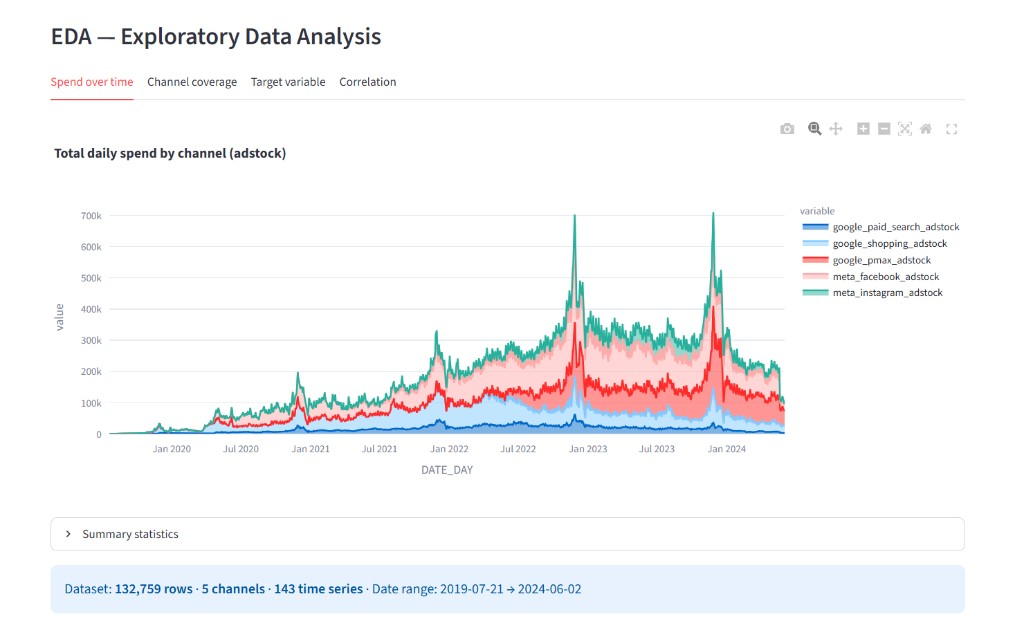
\includegraphics[width=\textwidth]{figures/figure2_eda.png}
  \caption{EDA --- total daily spend by channel (adstock), portfolio aggregate, July 2019--June 2024.}
\end{figure}

\section{Prediction Methodology and Results}

\subsection{Model form}

Each channel's contribution to weekly conversions is the saturation curve $f_c(s_c) = a_c(1 - e^{-b_c s_c})$ introduced in Section 3.2. Concavity is a deliberate \emph{design choice for the optimizer}: it guarantees every optimization subproblem downstream is convex, so the prediction layer and optimization engine are co-designed rather than bolted together.

\subsection{Estimation}

Curve parameters $(a_c, b_c)$ are fit by nonlinear least squares on weekly-aggregated training data. For the adstock model (Model C), curves are re-fit on steady-state effective spend at the holdout-selected decay rates, so the optimizer's input parameters are always consistent with the temporal assumption being modeled.

\subsection{Hyperparameter tuning via Bayesian Optimization}

The regularization weight and per-channel adstock decays cannot be chosen in-sample --- they are not separately identifiable, and each candidate configuration requires a full MMM refit plus holdout scoring, making the tuning objective an expensive black box. We therefore tune them with \textbf{Gaussian-Process Bayesian Optimization using Expected Improvement} over a 30-evaluation budget (5 random initial points + 25 EI-guided), scored on holdout $R^2$. The division of labor mirrors the course material: BO (Lecture 7) optimizes \emph{how the agent predicts}; gradient-based SLSQP optimizes \emph{how it allocates}, where the objective is cheap, smooth, and has an analytic gradient. Each algorithm is matched to the problem regime it was designed for.

\subsection{Fitted parameters and identification diagnostics}

\begin{center}
\begin{tabular}{lrrl}
\toprule
\textbf{Channel} & $a_c$ & $b_c$ & \textbf{Identification} \\
\midrule
google\_paid\_search & 9.01 & $3{\times}10^{-6}$ & Weak --- collinear with PMax \\
google\_shopping & 292{,}111.66 & $1{\times}10^{-6}$ & Strong \\
google\_pmax & 656{,}836.83 & ${\sim}0$ & Near-linear --- extrapolation risk \\
meta\_facebook & 767{,}739.98 & ${\sim}0$ & Near-linear --- extrapolation risk \\
meta\_instagram & 0.07 & $3{\times}10^{-6}$ & Weak --- collinear with Facebook \\
\bottomrule
\end{tabular}
\end{center}

Two structural findings are flagged by the agent rather than hidden. First, \textbf{within-platform multicollinearity}: brands scale Paid Search and PMax together, and Facebook and Instagram together, so the weaker member of each pair is not separately identifiable --- the regression assigns the shared effect to one channel. Second, the two strongest channels fit \textbf{near-linearly} within the observed spend range, meaning their fitted ceilings are extrapolations. Both caveats propagate into the recommendation language: the agent presents near-zero allocations on collinear channels as identification artifacts, not verdicts.

\subsection{Validation}

Holdout $R^2$ from the BO tuning run: [insert final holdout $R^2$, with the in-sample vs.\ holdout comparison from the BO logs]. The fitting path carries 11 dedicated unit tests; the curve fits shown above reproduce live in the app.

\begin{figure}[htbp]
  \centering
  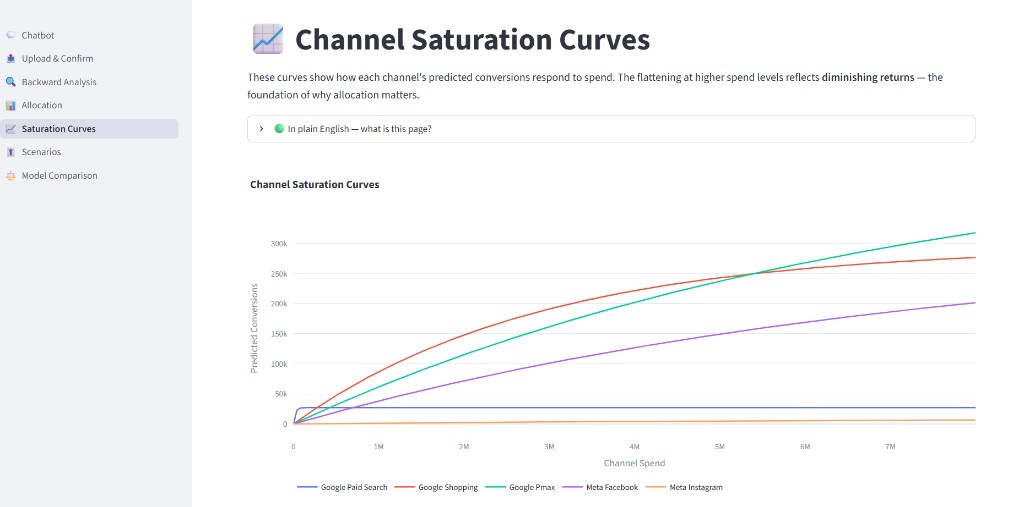
\includegraphics[width=\textwidth]{figures/figure3_saturation_curves.png}
  \caption{Channel saturation curves --- predicted conversions vs.\ channel spend. Google Shopping and PMax show strong scale; Paid Search and Instagram saturate at low spend (identification caveat).}
\end{figure}

\section{Optimization Model Formulation and Solution}

\subsection{Model A --- convex base}

\[
\max_{s} \sum_c a_c\left(1 - e^{-b_c s_c}\right)
\quad \text{s.t.} \quad \sum_c s_c \le B, \qquad 0 \le s_c \le u_c
\]

A concave objective over a polytope: every local optimum is global. We solve with \textbf{multistart SLSQP} (50 random starts), supplying the analytic gradient $\partial f_c / \partial s_c = a_c b_c e^{-b_c s_c}$, and \emph{verify the KKT conditions explicitly} on every solve:

\begin{enumerate}[nosep]
  \item \textbf{Primal feasibility} --- the allocation respects budget and bounds.
  \item \textbf{Stationarity} --- marginal returns are equalized across all channels spending strictly between their bounds; no profitable dollar transfer exists.
  \item \textbf{Dual feasibility} --- constraint multipliers are non-negative.
  \item \textbf{Complementary slackness} --- only binding constraints carry positive multipliers.
\end{enumerate}

The budget multiplier is reported to the user as the \textbf{shadow price} $\lambda_{\text{budget}}$: the predicted conversions gained per additional dollar of budget --- the single most decision-relevant number the optimizer produces.

\subsection{Model B --- activation thresholds (non-convex)}

The stakeholder modification makes each channel's feasible set $s_c \in \{0\} \cup [\kappa_c, u_c]$, a disjoint union; mixed-integer programming is disallowed by the assignment. A single local solve can converge on the wrong ON/OFF configuration. We restore a \emph{provable global optimum} by exhaustive enumeration: all $2^5 = 32$ activation patterns are generated, patterns whose minimum commitment $\sum_{c \in \text{ON}} \kappa_c$ exceeds $B$ are screened out, and a convex, KKT-verified SLSQP subproblem is solved within each surviving pattern. The best pattern wins. As a cross-check, a 50-start SLSQP attack on the unrestricted non-convex problem never beats the enumerated winner.

\subsection{Model C --- adstock carryover plus activation}

At steady state, geometric carryover implies effective spend $S^{\text{eff}}_c = s_c / (1 - \lambda_c)$. Model C maximizes $\sum_c a_c\,(1 - e^{-b_c s_c/(1-\lambda_c)})$ over Model B's feasible set, with curves re-fit at the holdout-selected decays. Carryover effectively discounts each channel's saturation rate, rewarding channels with long memory; the enumeration machinery runs unchanged.

\subsection{Solver configuration}

SciPy SLSQP; 50 multistarts; convergence tolerance $10^{-9}$; max 1{,}000 iterations. Every solve returns a single structured result object --- allocation, predicted conversions, KKT status, shadow price, baseline comparison, lift --- which is the integration contract consumed by every downstream page and by the explanation layer.

\section{Agent Architecture Description}

\subsection{The five components}

The agent implements the five components required by the project guidelines as one integrated pipeline:

\begin{center}
\begin{tabular}{ll}
\toprule
\textbf{Required component} & \textbf{Our implementation} \\
\midrule
1. Problem formulation & Guided 7-stage backward analysis + structured-brief parser (JSON schema) \\
2. Data collection \& preparation & Automated cleaning pipeline + weekly statistics layer (Section 4) \\
3. Prediction layer & Weekly MMM with BO-tuned hyperparameters (Section 5) \\
4. Optimization engine & Multistart SLSQP + activation-pattern enumeration, KKT-verified (Section 6) \\
5. Explanation \& validation & Plain-language rationale, sensitivity grids, diagnostics, benchmark comparison \\
\bottomrule
\end{tabular}
\end{center}

[Figure 5: Component map --- pipeline boxes with arrows from data preparation through prediction, optimization, and explanation.]

\subsection{End-to-end flow}

(1) The user uploads data and confirms the detected schema. (2) A \textbf{seven-stage backward analysis} walks from outcome identification through data quality, channel selection, response-curve logic, and constraint definition to an explicit optimization problem statement --- and the optimizer \emph{cannot run} until the user confirms that statement. This makes the backward mapping a living part of the product, not just a section of this report. (3) The pipeline fits curves and solves. (4--6) Results pages present the allocation against the baseline, the fitted curves, budget scenarios, and the Model A/B/C comparison, each with diagnostics.

\subsection{Configuration and runtime parameters}

Defaults (activation thresholds, decay rates, solver settings) live in a single configuration file; runtime truth lives in the app's session state. Every compute function in the stack --- ceiling computation, scale decisions, and the solvers themselves --- accepts runtime overrides for $\kappa$, $u_c$, and $B$, so when a stakeholder changes a threshold mid-conversation the entire chain re-evaluates consistently. Nothing is hard-coded twice.

\subsection{Guardrails: testable safety}

Chat input passes through a guardrail layer before any LLM sees it: scope enforcement (the agent answers only about this dataset and this decision), PII redaction (emails, phone numbers), and refusal of external-data requests and benchmark fabrication. Output is audited symmetrically: no unsourced statistics, no external-knowledge claims, mandatory data-source grounding. Every rule has a dedicated unit test covering block, redirect, pass-through, and redaction cases.

\subsection{LLM layer and graceful degradation}

The conversational agent runs on Anthropic Claude with a structured system prompt (identity, cognitive protocol, per-phase workflow instructions); the explanation layer's rationale generator uses Google Gemini. Critically, \textbf{no natural language ever reaches the solver} --- briefs are parsed into a strict JSON schema first, and all numbers shown to the user come from the deterministic pipeline, never from the LLM. Both LLM integrations degrade gracefully: with no API key, deterministic template output preserves full functionality, so the demo cannot break and the test suite runs key-free.

\subsection{Testing}

The full suite --- 197 passed, 2 intentionally skipped integration stubs --- runs with \texttt{pytest tests/} and no API key. Coverage spans the data pipeline, weekly statistics, archive handling, backward analysis, guardrails, MMM fitting, the optimizer, the baseline, BO tuning, and the explainer.

\section{Sensitivity and Scenario Analysis}

\subsection{Purpose and approach}

The project guidelines require the agent to report \emph{how the recommendation changes when key parameters shift}. Our primary sensitivity module lives on the app's \textbf{Sensitivity \& Scenario Analysis} page and answers a question every budget owner asks: \emph{what if my total budget were cut or increased?} Rather than perturbing curve parameters or activation thresholds on this page (those are handled separately on the Model A/B/C comparison page), we hold the fitted response curves $(a_c, b_c)$ and per-channel ceilings fixed and **re-solve the optimizer at each budget level**. This is a one-factor-at-a-time sensitivity on the total budget $B$ --- the same tornado-style logic used in the FreshChoice and airline case notebooks, applied to the constraint that binds most often in practice.

For each scenario the pipeline:
\begin{enumerate}[nosep]
  \item Computes a candidate budget $B' = m \times B_{\text{base}}$, where $m$ is a user-selected multiplier and $B_{\text{base}}$ is the budget from the confirmed optimization run.
  \item Calls the same SLSQP solver used on Page~3 (Model~A, KKT-verified) with unchanged $(a_c, b_c)$ and ceilings $u_c$.
  \item Records predicted conversions, the full allocation vector, and derived metrics (lift vs.\ base, conversions per \$1k).
\end{enumerate}

Because the objective is concave, each sub-solve is globally optimal for that budget; the sensitivity curve therefore traces the **efficient frontier of budget vs.\ conversions** implied by the fitted curves, not a heuristic extrapolation. When the budget rises, predicted conversions increase monotonically but **marginal efficiency** (conversions per additional \$1k) falls --- the diminishing-returns signature of concave saturation. When the budget falls, the optimizer may shift mix toward high-marginal-return channels; under large cuts, activation constraints on other pages can force channels OFF entirely.

\subsection{Scenario Settings: what each dial controls}

Three sidebar controls define the grid. None of them change the underlying model; they only define \emph{which budget levels to evaluate}:

\begin{center}
\begin{tabular}{p{3.2cm}p{2.2cm}p{8.5cm}}
\toprule
\textbf{Control} & \textbf{Example} & \textbf{Meaning} \\
\midrule
Min budget multiplier & 0.50 & Lower bound of the scenario range, expressed as a fraction of the base budget. \textbf{0.50} means ``simulate a 50\% budget cut'' ($B' = 0.5 \times B_{\text{base}}$). Slider range: 0.25--1.0. \\
Max budget multiplier & 2.00 & Upper bound of the scenario range. \textbf{2.00} means ``simulate doubling the budget'' ($B' = 2.0 \times B_{\text{base}}$). Slider range: 1.0--3.0. \\
Number of scenarios & 7 & How many evenly spaced budget levels to evaluate between min and max (inclusive). With min~0.50, max~2.00, and 7 points, the grid runs approximately 0.50$\times$, 0.75$\times$, 1.00$\times$ (base), 1.25$\times$, 1.50$\times$, 1.75$\times$, 2.00$\times$. If 1.00 is not hit exactly by the linspace, the base scenario is inserted automatically so the tornado chart always has a reference point. \\
\bottomrule
\end{tabular}
\end{center}

\textbf{Reading the headline metrics.} At portfolio scale ($B_{\text{base}}$ corresponding to the confirmed run), a typical seven-scenario grid produces:
\begin{center}
\begin{tabular}{lr}
\toprule
Base scenario (1.00$\times$) & 94{,}831.5 predicted conversions \\
Best scenario (2.00$\times$) & 152{,}346.7 (+57{,}515 vs.\ base) \\
Worst scenario (0.50$\times$) & 59{,}767.6 ($-$35{,}064 vs.\ base) \\
\bottomrule
\end{tabular}
\end{center}

These three numbers frame the conversation: doubling budget buys roughly 61\% more conversions; halving it loses roughly 37\%. The asymmetry (61\% gain vs.\ 37\% loss) is exactly concavity --- each marginal dollar buys less than the last, so proportional cuts and increases are not mirror images in percentage terms.

\subsection{Outputs and how to read them}

\textbf{Sensitivity tornado chart.} Horizontal bars show the \textbf{percent change in predicted conversions} relative to the base scenario. Green bars (budget increases) extend right; red bars (cuts) extend left. In the live run shown below, a 2.00$\times$ budget yields \textbf{+60.6\%} conversions vs.\ base; a 0.50$\times$ budget yields \textbf{$-$37.0\%}. The chart is ordered by magnitude so stakeholders immediately see which direction of budget change matters most. This is the project's primary tornado visualization --- single-factor, decision-relevant, and tied directly to re-optimized allocations rather than static curve shifts.

\begin{figure}[htbp]
  \centering
  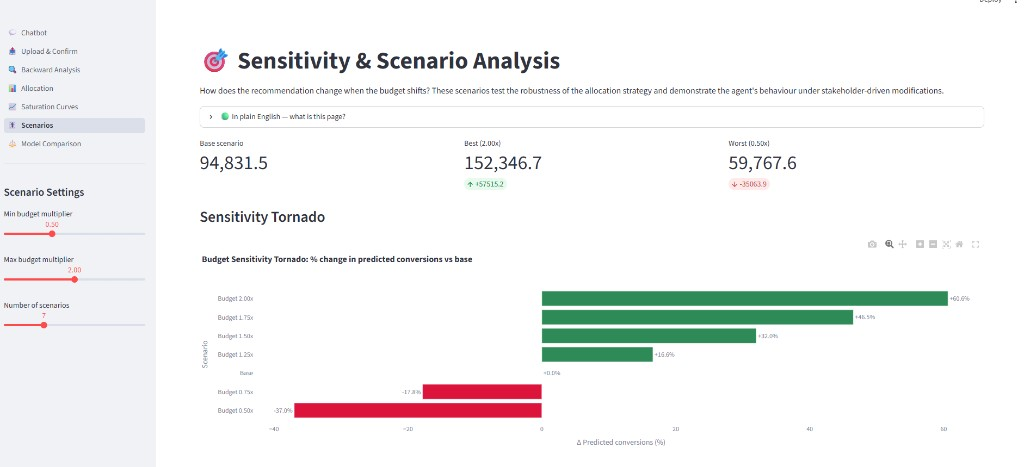
\includegraphics[width=\textwidth]{figures/sensitivity_tornado.png}
  \caption{Budget sensitivity tornado --- \% change in predicted conversions vs.\ base (portfolio scale; min multiplier 0.50, max 2.00, 7 scenarios).}
\end{figure}

\textbf{Allocation flow chart.} A stacked bar chart shows \emph{how the optimal mix shifts} as budget scales --- which channels absorb incremental dollars and which saturate first. This connects the abstract tornado to actionable mix decisions: a channel whose share grows across scenarios still has room on its curve; a channel whose share flatlines has hit diminishing returns or its ceiling $u_c$.

\textbf{Scenario summary table.} For each multiplier the table reports: budget \$ amount, predicted conversions, lift vs.\ base (\%), and \textbf{conversions per \$1k} (marginal efficiency at that budget level). The marginal-efficiency column is the headline number for stakeholder Q\&A: it captures whether the \emph{next} tranche of budget is worth funding. When conv/\$1k falls below the firm's unit-economics threshold, the grid identifies the budget level above which additional spend is no longer justified --- without requiring the executive to interpret KKT multipliers directly.

\subsection{Connection to course material}

This module implements the **Explanation and Validation Layer** requirement (Component~5): plain-language stress testing of the prescription. The approach mirrors **Lecture~2 --- Prediction to Prescription**: we do not ask ``what will conversions be if we spend 10\% more?'' with a single curve evaluation; we **re-optimize** at each budget because the optimal mix changes when the budget constraint moves (stationarity requires re-equalizing marginal returns). The diminishing marginal efficiency visible in the table is the numerical shadow price story from **Lecture~3 KKT** expressed in business units. The tornado format follows the sensitivity charts in the **FreshChoice and airline case notebooks**, adapted from parameter perturbation to budget perturbation because $B$ is the lever a marketing director actually controls.

\subsection{Activation-threshold sensitivity (companion analysis)}

Budget sensitivity holds $\kappa_c$ fixed. On the **Model A/B/C comparison** page, a complementary analysis re-runs Model~B at $\kappa \pm 20\%$ to test whether the winning ON/OFF channel set is robust to uncertainty in platform minimums. Together, the two analyses answer: (i)~``How sensitive is performance to my total budget?'' and (ii)~``How sensitive is the channel ON-set to assumed activation floors?'' --- covering the two stakeholder modifications from the benchmark specification.

\section{Benchmark Test Results and Comparison}

\subsection{Benchmark design}

The instructor's stakeholder modification serves as the benchmark: the team's own problem plus two frictions --- activation thresholds (Model B) and adstock carryover (Model C) --- with results compared on holdout weeks against the base Model A and a proportional-to-historical baseline.

\subsection{Model A headline}

Demonstration configuration, $B = \$50{,}000$ (chosen so activation effects are visible at demo scale):

\begin{center}
\begin{tabular}{lr}
\toprule
Predicted conversions (optimized) & 15{,}640.8 \\
Baseline conversions (proportional-to-historical) & 5{,}957.1 \\
\textbf{Lift vs.\ baseline} & \textbf{+162.6\%} \\
KKT status & pass \\
Budget shadow price $\lambda_{\text{budget}}$ & 0.3043 conv/\$ \\
Marginal efficiency & 312.8 conv/\$1k \\
\bottomrule
\end{tabular}
\end{center}

The lift is a \emph{reallocation gain} --- same budget, different distribution. The optimizer concentrates spend on Google Shopping, the channel whose curve identifies a strong concave response, while the baseline spreads dollars across collinear channels whose fitted incremental contribution is near zero.

Budget sensitivity results (tornado chart, allocation flow, marginal-efficiency table) are documented in Section~7; at demo scale (\$25k--\$100k), conversions per \$1k fall from 317.1 to 304.4 as budget rises.

\subsection{Model A / B / C comparison}

\begin{center}
\begin{tabular}{lccc}
\toprule
\textbf{Metric} & \textbf{Model A} & \textbf{Model B} & \textbf{Model C} \\
\midrule
Predicted conversions (holdout) & 15{,}640.8 & [insert result] & [insert result] \\
Shadow price $\lambda_{\text{budget}}$ & 0.3043 & [insert] & [insert] \\
Channels OFF / at $\kappa$ & none & [insert] & [insert] \\
\bottomrule
\end{tabular}
\end{center}

At portfolio scale ($B = \$831$k) no activation threshold binds and Model B coincides with Model A; at a \$90k stress scenario the activation mechanism switches channels off entirely rather than underfunding them --- the qualitative behavior the modification was designed to expose. A $\kappa \pm 20\%$ sweep tests whether the winning ON-set is robust to the assumed thresholds: [insert sweep outcome --- ON-set invariant, or which channels flip].

\subsection{Interpreting discrepancies}

Where our agent's answer differs from a human baseline, the difference traces to identification, not optimization: the solver provably finds the global optimum \emph{of the fitted curves}, so any disagreement is a statement about the prediction layer (collinearity, extrapolated ceilings) --- exactly the diagnostic the agent reports alongside its recommendation.

\begin{figure}[htbp]
  \centering
  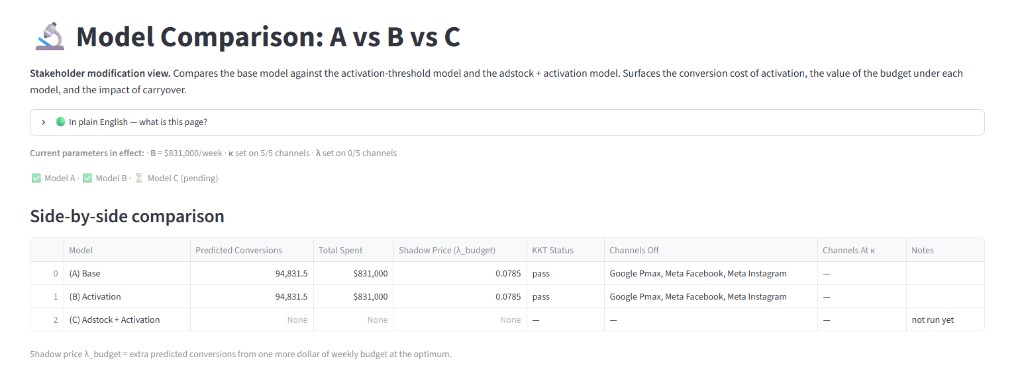
\includegraphics[width=\textwidth]{figures/figure6_model_comparison.png}
  \caption{Model A/B/C comparison at portfolio scale ($B = \$831{,}000$/week). Models A and B coincide; Model C pending adstock inputs.}
\end{figure}

\begin{figure}[htbp]
  \centering
  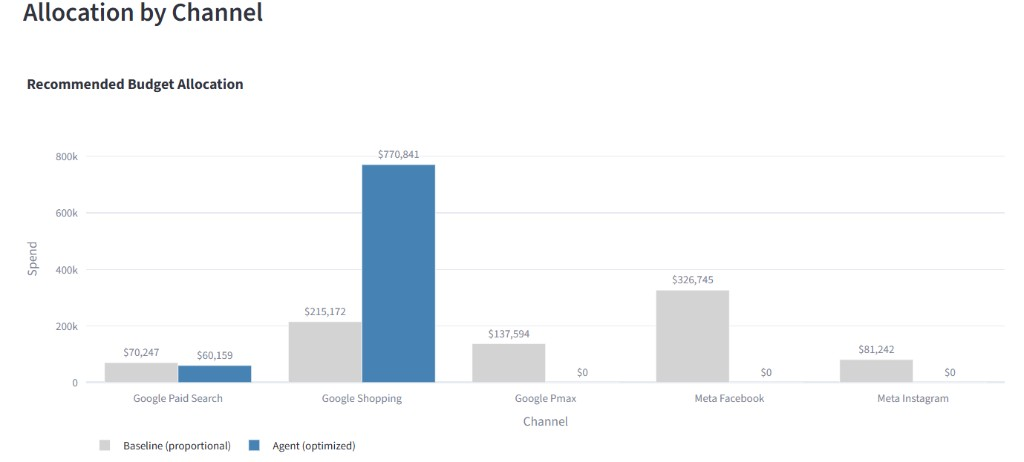
\includegraphics[width=\textwidth]{figures/figure7_allocation.png}
  \caption{Recommended allocation vs.\ proportional-to-historical baseline at portfolio scale.}
\end{figure}

\section{Managerial Recommendations}

\begin{enumerate}[nosep]
  \item \textbf{Reallocate before spending more.} At the same budget, redistributing dollars toward the highest marginal returns yields +162.6\% predicted conversions versus the proportional status quo. Concentrate the marginal dollar on Google Shopping until its marginal return falls to the shadow price or its ceiling binds.
  \item \textbf{Set the budget with the marginal-efficiency column.} If unit economics require at least 308 conversions per \$1k, the sensitivity grid caps the recommended budget near \$75k in the demo configuration; the same logic scales to the full portfolio.
  \item \textbf{Treat the collinear pairs as one decision each} until disambiguating evidence exists. Run geo-holdouts or platform lift studies on Paid Search vs.\ PMax and Facebook vs.\ Instagram; until then, near-zero allocations on the weaker members are identification artifacts, not verdicts.
  \item \textbf{Cap the near-linear channels managerially} (e.g., $1.2\times$ historical max) rather than trusting extrapolated ceilings.
  \item \textbf{Re-solve weekly.} The solver runs in milliseconds; refresh the recommendation every Monday as new data lands.
  \item \textbf{Platform minimums matter under cuts, not at scale.} At \$831k/week every channel clears its activation threshold; under a cut to \$90k the agent shows exactly which channels to switch off rather than underfund --- the kind of structural answer a heuristic cannot give.
\end{enumerate}

\section{Limitations and Future Improvements}

\textbf{Limitations} (acknowledged in-product, not just here): within-platform multicollinearity is structural to the dataset; near-linear fits make two channel ceilings extrapolations; the optimizer is single-period and the adstock bridge is the steady-state identity (transient dynamics unmodeled); curves are fit by squared-error loss rather than a decision-aware criterion; activation thresholds are stakeholder-supplied rather than estimated; modeling is at portfolio level rather than per-brand; narrative quality depends on LLM availability, though deterministic fallbacks preserve all function.

\textbf{Future improvements}, ordered by expected value: decision-aware curve fitting evaluated on holdout allocation regret; Bayesian MMM giving posterior distributions over $(a_c, b_c)$ and quantitative risk bands on the recommendation; posterior-based adstock estimation propagated through sample re-solves; designed experiments to disambiguate the collinear pairs; per-brand curves with a brand selector; multi-period optimization over a rolling horizon; contextual-bandit re-allocation in production; and mixed-integer formulation of the activation structure if the channel count grows beyond enumeration range ($2^n$ is trivial at $n=5$, untenable at $n=20$).

\section*{AI Usage Disclosure}

Generative AI tools were used in two distinct roles, disclosed per course policy. \emph{As a development tool:} Cursor (Claude-based) assisted with code scaffolding, test generation, and documentation drafting; all model formulations, data decisions, and business interpretations were specified, reviewed, and validated by the team, and every component is covered by team-written acceptance criteria and tests. \emph{As a product component:} the deployed agent uses Anthropic Claude for conversation and Google Gemini for rationale generation, with guardrails and deterministic fallbacks as described in Section~6. No LLM output enters any numerical computation.

\section*{Team Contributions}

All members are jointly responsible for the full system; primary contribution areas were:

\begin{center}
\begin{tabular}{ll}
\toprule
\textbf{Member} & \textbf{Primary contributions} \\
\midrule
Ana Valderrama & Data pipeline, weekly statistics layer, backward-analysis flow, guardrails, agent prompts \\
Gregory Sapp & MMM prediction layer, weekly frequency support, curve-fit validation \\
Meghna Advani & Optimization engine (Models A/B/C), KKT verification, BO tuning, baseline \\
Piyush Sandhikar & Agent orchestration, problem-formulation module, LLM integration \\
Vikhyat Koppal & Explanation layer, results and scenario pages, sensitivity visualizations \\
\bottomrule
\end{tabular}
\end{center}

\vspace{0.5em}
\noindent\textbf{Grading dimension map.} Problem Formulation: Sections 1--2. Data and Prediction: Sections 3--4. Optimization Model: Sections 5, 8, and 9. Agent Design and Integration: Section 6. Presentation and Communication: Executive Summary, Section 7 (sensitivity), and Sections 9--10.

\end{document}
